\documentclass[aspectratio=169,11pt]{beamer}

% ============================================================
% THEME & COLOURS (matched to GDP PowerPoint)
% ============================================================
\usetheme{default}
\usecolortheme{default}
\setbeamertemplate{navigation symbols}{}

\definecolor{gdpPurple}{HTML}{633E88}
\definecolor{gdpDarkBlue}{HTML}{0C406D}
\definecolor{gdpNavy}{HTML}{091932}
\definecolor{gdpOrange}{HTML}{DD7A0F}
\definecolor{gdpSlate}{HTML}{3B4950}
\definecolor{gdpLightGray}{HTML}{E7E6E6}
\definecolor{gdpBurgundy}{HTML}{820E21}

\setbeamercolor{background canvas}{bg=white}
\setbeamercolor{normal text}{fg=gdpSlate}
\setbeamercolor{frametitle}{fg=gdpPurple,bg=white}
\setbeamercolor{framesubtitle}{fg=gdpDarkBlue,bg=white}
\setbeamercolor{title}{fg=gdpPurple}
\setbeamercolor{subtitle}{fg=gdpDarkBlue}
\setbeamercolor{author}{fg=gdpSlate}
\setbeamercolor{institute}{fg=gdpSlate}
\setbeamercolor{date}{fg=gdpSlate}
\setbeamercolor{item}{fg=gdpDarkBlue}
\setbeamercolor{subitem}{fg=gdpPurple}
\setbeamercolor{block title}{fg=white,bg=gdpDarkBlue}
\setbeamercolor{block body}{fg=gdpSlate,bg=gdpLightGray!30}
\setbeamercolor{block title alerted}{fg=white,bg=gdpBurgundy}
\setbeamercolor{block body alerted}{fg=gdpSlate,bg=gdpLightGray!30}
\setbeamercolor{footline}{fg=gdpSlate}

\usepackage{helvet}
\renewcommand{\familydefault}{\sfdefault}
\usepackage{amsmath,amssymb,graphicx,booktabs,array,tikz}
\usepackage{pifont}
\newcommand{\cmark}{\ding{51}}
\newcommand{\xmark}{\ding{55}}

\setlength{\tabcolsep}{3pt}
\setbeamertemplate{itemize/enumerate body begin}{\small}
\setbeamertemplate{itemize/enumerate subbody begin}{\footnotesize}
\addtolength{\leftmargini}{-0.3cm}
\addtolength{\leftmarginii}{-0.2cm}

\setbeamertemplate{frametitle}{%
  \vspace{0.2cm}
  \textbf{\large\insertframetitle}
  \vspace{0.05cm}
  \par\textcolor{gdpDarkBlue}{\rule{\textwidth}{1.2pt}}
  \vspace{-0.3cm}
}

\setbeamertemplate{footline}{%
  \leavevmode%
  \hbox{%
    \begin{beamercolorbox}[wd=.333\paperwidth,ht=2.5ex,dp=1ex,leftskip=0.3cm]{footline}%
      \insertshortauthor
    \end{beamercolorbox}%
    \begin{beamercolorbox}[wd=.333\paperwidth,ht=2.5ex,dp=1ex,center]{footline}%
      \insertshorttitle
    \end{beamercolorbox}%
    \begin{beamercolorbox}[wd=.333\paperwidth,ht=2.5ex,dp=1ex,rightskip=0.3cm]{footline}%
      \insertframenumber{}
    \end{beamercolorbox}%
  }%
}

\setbeamertemplate{title page}{
  \vspace{1.5cm}
  \begin{center}
    {\Huge\bfseries\textcolor{gdpPurple}{\inserttitle}}\\[0.4cm]
    {\Large\textcolor{gdpDarkBlue}{\insertsubtitle}}\\[1.2cm]
    {\large\textcolor{gdpSlate}{\insertauthor}}\\[0.3cm]
    {\normalsize\textcolor{gdpSlate}{\insertinstitute}}\\[0.3cm]
    {\normalsize\textcolor{gdpSlate}{\insertdate}}
  \end{center}
}

\title{From Thermal Air Layers to JCA Porous Media}
\subtitle{Model Pivot for Analog Wave Computation}
\author{MSc Individual Research Project}
\institute{Cranfield University\hspace{0.3cm}|\hspace{0.3cm}Supervisors: Prof. Weisi Guo, Prof. Takis Tsoutsanis}
\date{14 June 2026}

\begin{document}

% ============================================================
\begin{frame}[plain]
  \titlepage
\end{frame}

% ============================================================
\begin{frame}{Where We Are}
 
  \vspace{0.3cm}
  \textbf{Two paths examined:}
  \begin{enumerate}
    \item \textbf{Thermal air layers:} static temperature field changes local sound speed $c(T)$ and density $\rho(T)$.
    \item \textbf{Rigid-frame porous media:} Johnson-Champoux-Allard (JCA) equivalent fluid gives frequency-dependent damping and dispersion.
  \end{enumerate}

  \vspace{0.3cm}
  \textbf{Today:} why the thermal path is abandoned, and why the JCA Helmholtz model is now the forward model.
\end{frame}

% ============================================================
\begin{frame}{Computational Domain}
  \begin{center}
  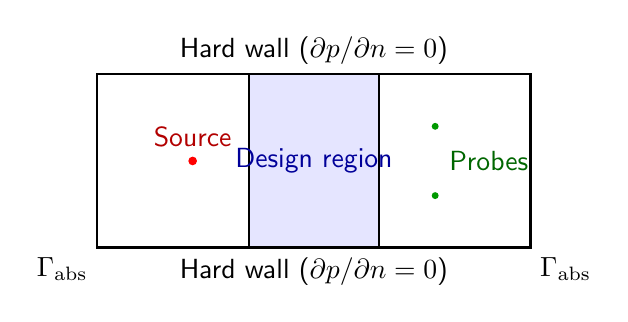
\begin{tikzpicture}[scale=0.55]
    \draw[thick] (0,0) rectangle (10,4);
    \fill[blue!10] (3.5,0) rectangle (6.5,4);
    \draw[thick] (3.5,0) rectangle (6.5,4);
    \node[blue!60!black] at (5,2) {Design region};
    \fill[red] (2.2,2) circle (0.1);
    \node[red!70!black, above] at (2.2,2.1) {Source};
    \fill[green!60!black] (7.8,1.2) circle (0.08);
    \fill[green!60!black] (7.8,2.8) circle (0.08);
    \node[green!40!black, right] at (7.9,2) {Probes};
    \node[above] at (5,4) {Hard wall ($\partial p/\partial n = 0$)};
    \node[below] at (5,0) {Hard wall ($\partial p/\partial n = 0$)};
    \node[below left] at (0,0) {$\Gamma_\mathrm{abs}$};
    \node[below right] at (10,0) {$\Gamma_\mathrm{abs}$};
  \end{tikzpicture}
  \end{center}

  \vspace{0.2cm}
  \footnotesize
  \begin{itemize}
    \item 2-D duct / waveguide: hard walls top/bottom, absorbing ends.
    \item Source injects waves from the left; probes record the output field.
    \item The design region is the subdomain whose acoustic properties we control.
    \item Objective: shape the wave field so the right signal reaches the right probe.
  \end{itemize}

  \vspace{0.1cm}
  \textcolor{gdpDarkBlue}{\small Domain size: $800 \times 100$~mm, grid $400 \times 50$, $\Delta x = 2$~mm.}
\end{frame}

% ============================================================
\begin{frame}{Thermal Path: Concept and Governing Equations}
  \textbf{Idea:} a laser heating pattern $T(\mathbf{x})$ rewrites the acoustic properties of air; the temperature field becomes the ``weight matrix.''

  \vspace{0.15cm}
  Steady-state heat conduction with volumetric source $\sigma$:
  \[
    \nabla^2 T = -\frac{\sigma}{D_\text{thermal}}
  \]
  For an ideal gas:
  \[
    c(T) = c_0\sqrt{\frac{T}{T_0}}, \qquad
    \rho(T) = \rho_0\frac{T_0}{T}
  \]

  \vspace{0.05cm}
  \begin{block}{\footnotesize What we tested}
    \scriptsize
    \begin{itemize}
      \item 1D transfer matrix for hot-air stacks
      \item 2D first-order FDTD with $c(T)$
    \end{itemize}
  \end{block}
\end{frame}

% ============================================================
\begin{frame}{1D Transfer-Matrix Result}
  \begin{columns}[T]
    \begin{column}{0.58\textwidth}
      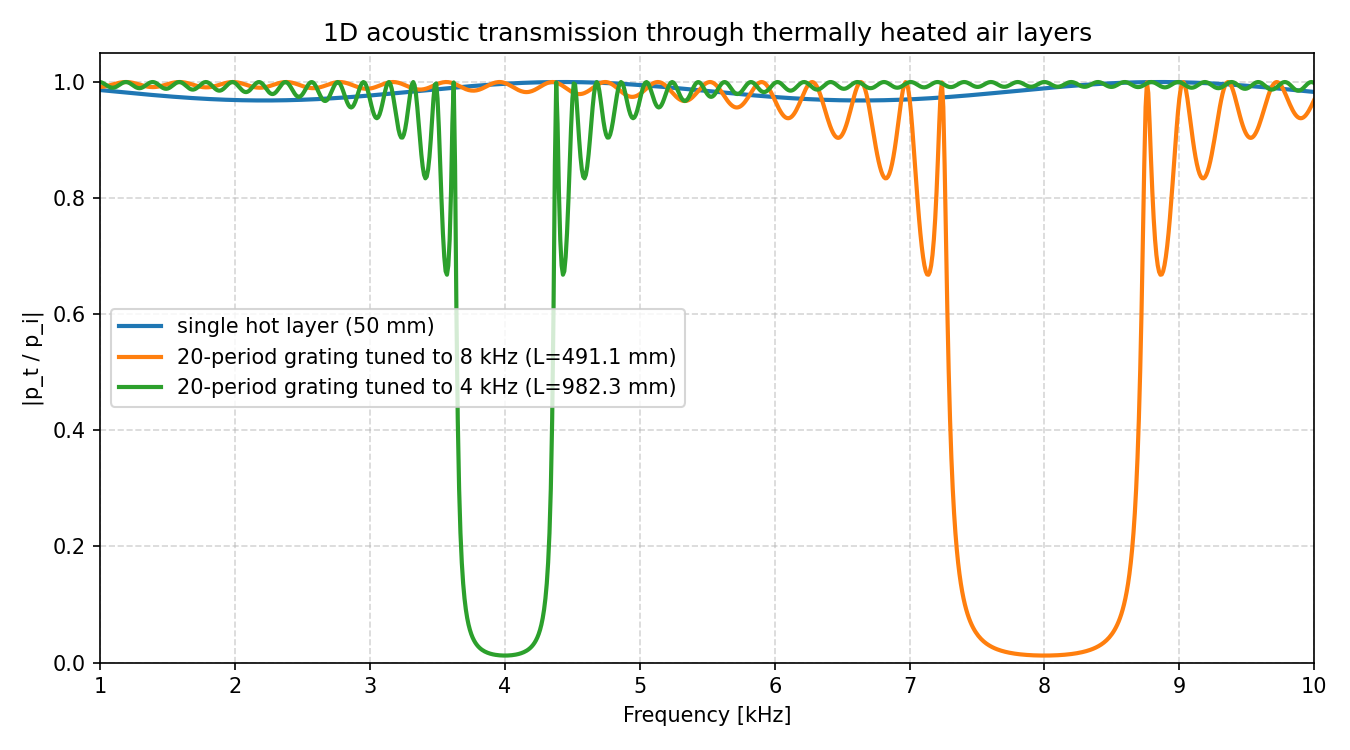
\includegraphics[width=\textwidth]{../Analysis/figures/thermal_1d_transmission.png}
    \end{column}
    \begin{column}{0.38\textwidth}
      \footnotesize
      \textbf{Key observations:}
      \begin{itemize}
        \item A single 50~mm hot layer is essentially transparent.
        \item Strong stop bands require a multi-period Bragg grating.
        \item 20 periods at 8~kHz $\Rightarrow$ 491~mm.
        \item 20 periods at 4~kHz $\Rightarrow$ 982~mm.
      \end{itemize}

      \vspace{0.2cm}
      \textcolor{gdpBurgundy}{\textbf{Conclusion:} useful acoustic contrast only appears at device lengths incompatible with a compact wave computer.}
    \end{column}
  \end{columns}
\end{frame}

% ============================================================
\begin{frame}{2D FDTD Confirmation}
  \begin{columns}[T]
    \begin{column}{0.50\textwidth}
      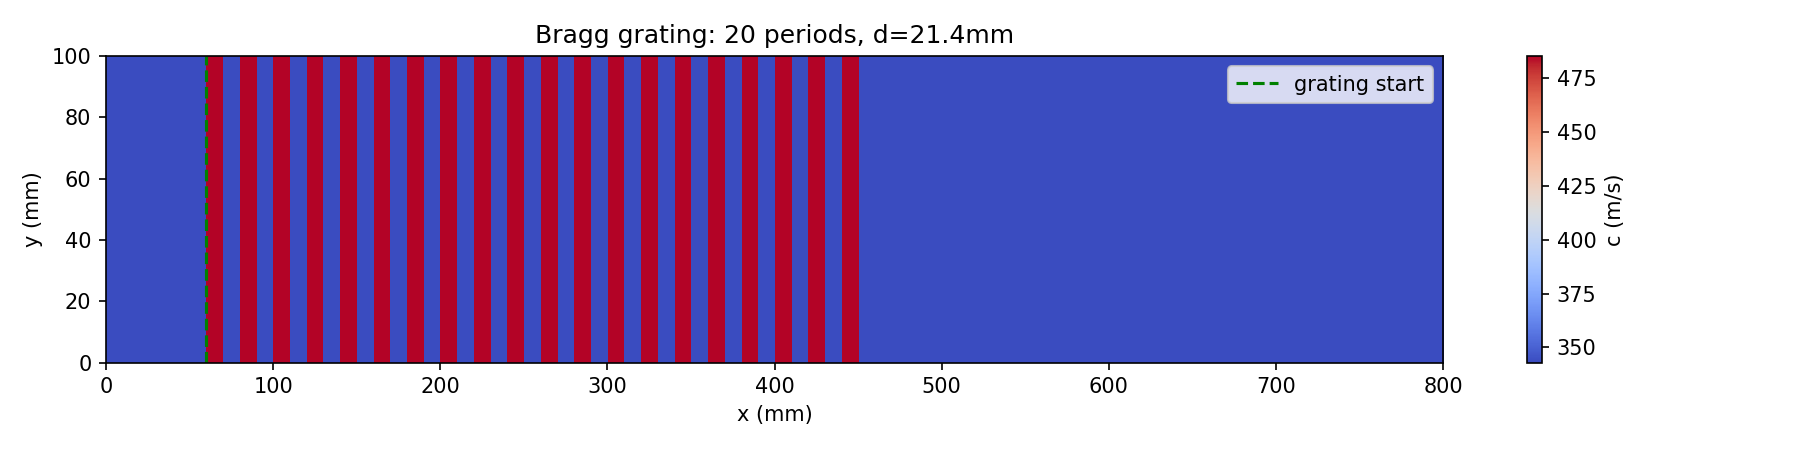
\includegraphics[width=\textwidth]{../bragg_grating_layout.png}
      \\[-0.1cm]
      {\footnotesize 20-period thermal grating at 8~kHz (scale in mm).}
    \end{column}
    \begin{column}{0.46\textwidth}
      \footnotesize
      \textbf{2D time-domain experiments:}
      \begin{itemize}
        \item A useful band gap needs many periods.
        \item At speech-band frequencies (2--4~kHz) the grating is 0.3--0.5~m long.
        \item Thermal diffusion blurs fine features before strong contrast can be built.
      \end{itemize}

      \vspace{0.2cm}
      \begin{block}{\footnotesize Why this path is dropped}
        \footnotesize
        Weak per-wavelength contrast $\;+\;$ large required size $\;+\;$ thermal blur make thermal air layers an impractical substrate.
      \end{block}
    \end{column}
  \end{columns}
\end{frame}

% ============================================================
\begin{frame}{New Forward Model: JCA Equivalent-Fluid Helmholtz}
  \textbf{Medium:} rigid-frame porous scaffold saturated with air, described by the Johnson-Champoux-Allard (JCA) model.

  \vspace{0.2cm}
  Time-harmonic pressure $p(\mathbf{x})$ satisfies
  \begin{equation}
    \nabla \cdot \left( \frac{1}{\tilde{\rho}(\omega,\mathbf{x})} \nabla p \right)
    + \frac{\omega^2}{\tilde{K}(\omega,\mathbf{x})}\, p
    = S(\omega)\,\delta(\mathbf{x}-\mathbf{x}_s).
    \label{eq:jca_helmholtz}
  \end{equation}

  \vspace{0.1cm}
  \begin{itemize}
    \item $\tilde{\rho}$ and $\tilde{K}$ are \textbf{complex, frequency-dependent} effective density and bulk modulus.
    \item Coefficients vary with position; material interfaces are handled inside the divergence operator.
    \item The rigid-frame assumption keeps the model tractable while still capturing the physics that matters for wave computation.
  \end{itemize}
\end{frame}

% ============================================================
\begin{frame}{JCA Effective Properties}
  \footnotesize
  \textbf{Effective density} (Johnson-Koplik-Dashen + viscous correction)
  \begin{equation}
    \tilde{\rho}(\omega,\mathbf{x}) = \frac{\rho_0\alpha_\infty}{\phi}
    \left[
      1 + \frac{\sigma\phi}{j\omega\rho_0\alpha_\infty}
      \sqrt{1 + j\frac{4\alpha_\infty^2\eta\rho_0\omega}{\sigma^2\phi^2\Lambda^2}}
    \right].
  \end{equation}

  \vspace{0.1cm}
  \textbf{Effective bulk modulus} (Champoux-Allard thermal correction)
  \begin{equation}
    \tilde{K}(\omega,\mathbf{x}) = \frac{\gamma P_0}{\phi}
    \left[
      \gamma - \frac{\gamma-1}{1 + \dfrac{8\eta}{j\omega\rho_0 Pr\,\Lambda'^2}
      \sqrt{1 + j\dfrac{\omega\rho_0 Pr\,\Lambda'^2}{16\eta}}}
    \right]^{-1}.
  \end{equation}

  \vspace{0.1cm}
  From these:
  \[
    k(\omega,\mathbf{x}) = \omega\sqrt{\frac{\tilde{\rho}}{\tilde{K}}}, \qquad
    Z_c(\omega,\mathbf{x}) = \sqrt{\tilde{\rho}\,\tilde{K}}.
  \]
\end{frame}

% ============================================================
\begin{frame}{Why JCA? Why Frequency Domain?}
  \begin{columns}[T]
    \begin{column}{0.55\textwidth}
      \textbf{Why the JCA equivalent-fluid model?}
      \begin{itemize}
        \item Strong scattering and damping per wavelength $\Rightarrow$ compact devices.
        \item \textbf{Three continuous design knobs} per block: porosity $\phi$, flow resistivity $\sigma$, tortuosity $\alpha_\infty$.
        \item Natural impedance contrast between air and porous regions.
        \item Well validated for rigid-frame foams, sintered metals, and 3D-printed lattices.
      \end{itemize}
    \end{column}
    \begin{column}{0.42\textwidth}
      \textbf{Why frequency-domain Helmholtz?}
      \begin{itemize}
        \item Direct access to the steady-state transfer function at each frequency.
        \item Avoids long time-domain transients in highly damped porous media.
        \item Natural fit for frequency-routing / classification tasks.
      \end{itemize}
    \end{column}
  \end{columns}

  \vspace{0.3cm}
  %\textcolor{gdpDarkBlue}{\small The model is linear; nonlinearity is not required for the core proof-of-concept wave-computing task.}
\end{frame}

% ============================================================
\begin{frame}{Boundary Conditions}
  \textbf{Domain layout:} a 2D duct / waveguide containing the design region.

  \vspace{0.1cm}
  \begin{columns}[T]
    \begin{column}{0.55\textwidth}
      \footnotesize
      \setlength{\itemsep}{2pt}
      \begin{itemize}
        \item \textbf{Internal source:} $S(\omega)\,\delta(\mathbf{x}-\mathbf{x}_s)$ injects time-harmonic pressure inside the domain.
        \item \textbf{Left / right ends:} absorbing boundary $\Gamma_\text{abs}$ (PML or ABC) to mimic free-field radiation.
        \item \textbf{Top / bottom:} hard-wall boundary $\Gamma_\text{wall}$ ($\partial p/\partial n = 0$).
        \item \textbf{Porous--air interfaces:} continuity of pressure and normal volume velocity is automatic because the JCA coefficients remain inside the divergence operator.
      \end{itemize}
    \end{column}
    \begin{column}{0.42\textwidth}
      \begin{block}{\footnotesize Why this choice?}
        \scriptsize
        Mimics a realistic experimental waveguide, prevents reflected energy from contaminating the probe readouts, and avoids explicit interface matching conditions.
      \end{block}
    \end{column}
  \end{columns}
\end{frame}

% ============================================================
\begin{frame}{Design Parameterisation}
  \textbf{Design region:} divided into coarse rectangular blocks. Each block carries three bounded variables:
  \[
    \phi_b \in [0.30,\,0.95], \qquad
    \sigma_b \in [0,\,10^5]\;\text{Pa\,s\,m}^{-2}, \qquad
    \alpha_{\infty,b} \in [1.0,\,2.5].
  \]

  \vspace{0.2cm}
  Viscous and thermal characteristic lengths are fixed:
  \[
    \Lambda = 30~\mu\text{m}, \qquad \Lambda' = 60~\mu\text{m}.
  \]

  \vspace{0.2cm}
  \textbf{Why block-wise?}
  \begin{itemize}
    \item Reduces the design space from thousands of grid points to tens or hundreds of variables.
    \item Produces interpretable, manufacturable porous-block layouts.
    \item Suppresses fine checkerboard patterns without penalty terms.
  \end{itemize}
\end{frame}

% ============================================================
\begin{frame}{Closest Work}
  a 2D spatially varying rigid-frame porous medium, parameterised by $(\phi,\sigma,\alpha_\infty)$ and designed by inverse methods for an analog wave-computing task, appears to be novel, But at this point I don't know, anything at all.

  \vspace{0.2cm}
  \footnotesize
  \begin{table}
    \centering
    \renewcommand{\arraystretch}{1.05}
    \begin{tabular}{@{}>{\raggedright}p{3.4cm}>{\raggedright}p{4.0cm}>{\raggedright\arraybackslash}p{4.8cm}@{}}
      \toprule
      \textbf{Reference} & \textbf{What they do} & \textbf{How this project differs} \\
      \midrule
      Pan et al.\ 2023 & 2D metaporous absorption via CNN--GA & Goal is absorption, not wave computation \\
      Boulvert et al.\ 2019 & 1D graded JCAL broadband absorber & One-dimensional, absorption objective \\
      Parsa et al.\ 2022 & Evolved acoustic logic gates in granular media & Granular, not continuous porous medium \\
      \bottomrule
    \end{tabular}
  \end{table}
\end{frame}

% ============================================================
\begin{frame}{Open Questions for Today}
  \textbf{Remaining decisions before optimisation begins:}
  \begin{enumerate}
    \item \textbf{Wave-computing task:} XOR logic gate, frequency binary classifier, spatial source classifier, or binary vowel classifier?
    \item \textbf{PML / absorbing layer:} thickness and reflection level to accept.
    \item \textbf{Validation benchmark:} uniform JCA slab via transfer matrix.
  \end{enumerate}

  \vspace{0.3cm}
  %\textcolor{gdpDarkBlue}{\small Recommendation: choose the simplest task that still demonstrates non-trivial 2D wave routing (e.g.\ frequency binary classifier or XOR gate).}
\end{frame}

% ============================================================
\begin{frame}{Summary}
  \begin{itemize}
    \item \textbf{Thermal air layers} give only weak per-wavelength contrast; useful filtering requires impractically large multi-period gratings.
    \item \textbf{JCA porous media} replace temperature with material parameters $\phi$, $\sigma$, $\alpha_\infty$, giving strong compact scattering and damping.
    \item \textbf{Forward model:} frequency-domain JCA Helmholtz with internal source, absorbing ends, and hard-wall sides.
    \item \textbf{Design space:} coarse blocks of porosity, flow resistivity, and tortuosity; characteristic lengths fixed.
    \item \textbf{Next step:} select the wave-computing demonstration and run the first optimisation.
  \end{itemize}

  \vspace{0.4cm}
  \begin{center}
    \Large\textbf{\textcolor{gdpPurple}{Questions / Discussion}}
  \end{center}
\end{frame}

\end{document}
